%% For double-blind review submission, w/o CCS and ACM Reference (max submission space)
\documentclass[acmsmall,review,anonymous]{acmart}\settopmatter{printfolios=true,printccs=false,printacmref=false}
%% For double-blind review submission, w/ CCS and ACM Reference
%\documentclass[acmsmall,review,anonymous]{acmart}\settopmatter{printfolios=true}
%% For single-blind review submission, w/o CCS and ACM Reference (max submission space)
%\documentclass[acmsmall,review]{acmart}\settopmatter{printfolios=true,printccs=false,printacmref=false}
%% For single-blind review submission, w/ CCS and ACM Reference
%\documentclass[acmsmall,review]{acmart}\settopmatter{printfolios=true}
%% For final camera-ready submission, w/ required CCS and ACM Reference
%\documentclass[acmsmall]{acmart}\settopmatter{}


%% Journal information
%% Supplied to authors by publisher for camera-ready submission;
%% use defaults for review submission.
% \acmJournal{PACMPL}
% \acmVolume{1}
% \acmNumber{CONF} % CONF = POPL or ICFP or OOPSLA
% \acmArticle{1}
% \acmYear{2018}
% \acmMonth{1}
% \acmDOI{} % \acmDOI{10.1145/nnnnnnn.nnnnnnn}
% \startPage{1}

%% Copyright information
%% Supplied to authors (based on authors' rights management selection;
%% see authors.acm.org) by publisher for camera-ready submission;
%% use 'none' for review submission.
\setcopyright{none}
%\setcopyright{acmcopyright}
%\setcopyright{acmlicensed}
%\setcopyright{rightsretained}
%\copyrightyear{2018}           %% If different from \acmYear

%% Bibliography style
\bibliographystyle{ACM-Reference-Format}
%% Citation style
%% Note: author/year citations are required for papers published as an
%% issue of PACMPL.
\citestyle{acmauthoryear}   %% For author/year citations


% %% Some recommended packages.
% \usepackage{booktabs}   %% For formal tables:
%                         %% http://ctan.org/pkg/booktabs
\usepackage{subcaption} %% For complex figures with subfigures/subcaptions
                        %% http://ctan.org/pkg/subcaption
\usepackage{wrapfig}

\usepackage{ifthen}
\usepackage{pgf}
\usepackage{ulem}
\usepackage{tikz}
\usepackage{tikzpeople}
\usetikzlibrary{backgrounds}
\usetikzlibrary{fit}
\usetikzlibrary{calc}
\usetikzlibrary{positioning}
\usetikzlibrary{patterns}
\usetikzlibrary{decorations.pathreplacing}
\usetikzlibrary{arrows,shapes}
\usepackage{amssymb}

% Active adversary
\newcommand{\actadv}[4][]{
  \ifthenelse{\equal{#1}{}}{
    \draw[fill=white] #2 rectangle #3 node[pos=.5] {};
    \draw ($#2 + (2.25,1.5)$) node[devil,mirrored,minimum size=1cm] {};
    \draw[fill=white, fill opacity=0.5] #2 rectangle #3 node[pos=.5] {};
    \draw #2 rectangle #3 node[pos=.5,align=center] {\footnotesize #4};
  }{
    \onlyenv<#1>
    \draw[fill=white] #2 rectangle #3 node[pos=.5] {};
    \draw ($#2 + (3,1.5)$) node[devil,mirrored,minimum size=1cm] {};
    \draw[fill=white, fill opacity=0.5] #2 rectangle #3 node[pos=.5] {};
    \draw #2 rectangle #3 node[pos=.5] {\footnotesize #4};
    \endonlyenv
  }
}

% Inactive adversary
\newcommand{\inactadv}[4][]{
  \ifthenelse{\equal{#1}{}}{
    \draw[fill=white] #2 rectangle #3 node[pos=.5] {};
    \draw ($#2 + (2.25,1.5)$) node[devil,mirrored,minimum size=1cm] {};
    \draw[fill=white, fill opacity=0.4] #2 rectangle #3 node[pos=.5] {};
    \draw[fill=gray, fill opacity=0.5] #2 rectangle #3 node[pos=.5] {};
    \draw #2 rectangle #3 node[pos=.5] {\footnotesize #4};
  }{
    \onlyenv<#1>
    \draw[fill=white] #2 rectangle #3 node[pos=.5] {};
    \draw ($#2 + (3,1.5)$) node[devil,mirrored,minimum size=1cm] {};
    \draw[fill=white, fill opacity=0.4] #2 rectangle #3 node[pos=.5] {};
    \draw[fill=gray, fill opacity=0.5] #2 rectangle #3 node[pos=.5] {};
    \draw #2 rectangle #3 node[pos=.5] {\footnotesize #4};
    \endonlyenv
  }
}

% Active stack frame
\newcommand{\actsf}[4][]{
  \ifthenelse{\equal{#1}{}}{
    \draw[fill=white] #2 rectangle #3 node[pos=.5] {\footnotesize #4};
  }{
   \draw<#1>[fill=white] #2 rectangle #3 node[pos=.5] {#4};
 }
}

% Inactive stack frame
\newcommand{\inactsf}[4][]{
  \ifthenelse{\equal{#1}{}}{
    \draw[fill=white] #2 rectangle #3 node[pos=.5] {};
    \draw[fill=gray, fill opacity=0.5] #2 rectangle #3 node[pos=.5] {};
    \draw #2 rectangle #3 node[pos=.5] {\footnotesize #4};
  }{
    \draw<#1>[fill=white] #2 rectangle #3 node[pos=.5] {};
    \draw<#1>[fill=gray, fill opacity=0.5] #2 rectangle #3 node[pos=.5] {};
    \draw<#1> #2 rectangle #3 node[pos=.5] {\footnotesize #4};
  }
}

\newcommand{\capbrace}[3][sp1]{
  \draw [decorate,decoration={brace,amplitude=10pt,mirror,raise=4pt},yshift=0pt]
  #2 -- #3 node[draw=black] (#1) [black,midway,xshift=0.8cm] {};

}

\newcommand{\stdstackstart}{
  \scope
    \clip (-.1,-.1) rectangle (4.6,11.1);
    \fill[fill=white] (0,0) rectangle (4.5,11);
    \draw (0,0) -- (0,11);
    \draw (4.5,0) -- (4.5,11);
    \draw[fill=gray!50] (0,-.5) rectangle (4.5,2)
    node[pos=.5,color=black,align=center,yshift=0.1cm] {\footnotesize Higher
      stack\\\footnotesize frames...};
  \endscope
  % \draw[->] (-2,0) -- node[midway,sloped,above] {stack grows upward} (-2,15);
  \draw (-1.5,0) node {};
  \draw (-1.5,15) node {};
}


% stolen from https://tex.stackexchange.com/questions/14225/is-there-the-easiest-way-to-toggle-show-hide-navigational-grids-in-tikz/14230
\makeatletter
\newif\if@showgrid@grid
\newif\if@showgrid@left
\newif\if@showgrid@right
\newif\if@showgrid@below
\newif\if@showgrid@above
\tikzset{%
    every show grid/.style={},
    show grid/.style={execute at end picture={\@showgrid{grid=true,#1}}},%
    show grid/.default={true},
    show grid/.cd,
    labels/.style={font={\sffamily\small},help lines},
    xlabels/.style={},
    ylabels/.style={},
    keep bb/.code={\useasboundingbox (current bounding box.south west) rectangle (current bounding box.north west);},
    true/.style={left,below},
    false/.style={left=false,right=false,above=false,below=false,grid=false},
    none/.style={left=false,right=false,above=false,below=false},
    all/.style={left=true,right=true,above=true,below=true},
    grid/.is if=@showgrid@grid,
    left/.is if=@showgrid@left,
    right/.is if=@showgrid@right,
    below/.is if=@showgrid@below,
    above/.is if=@showgrid@above,
    false,
}

\def\@showgrid#1{%
    \begin{scope}[every show grid,show grid/.cd,#1]
    \if@showgrid@grid
    \begin{pgfonlayer}{background}
    \draw [help lines]
        (current bounding box.south west) grid
        (current bounding box.north east);
%
    \pgfpointxy{1}{1}%
    \edef\xs{\the\pgf@x}%
    \edef\ys{\the\pgf@y}%
    \pgfpointanchor{current bounding box}{south west}
    \edef\xa{\the\pgf@x}%
    \edef\ya{\the\pgf@y}%
    \pgfpointanchor{current bounding box}{north east}
    \edef\xb{\the\pgf@x}%
    \edef\yb{\the\pgf@y}%
    \pgfmathtruncatemacro\xbeg{ceil(\xa/\xs)}
    \pgfmathtruncatemacro\xend{floor(\xb/\xs)}
    \if@showgrid@below
    \foreach \X in {\xbeg,...,\xend} {
        \node [below,show grid/labels,show grid/xlabels] at (\X,\ya) {\X};
    }
    \fi
    \if@showgrid@above
    \foreach \X in {\xbeg,...,\xend} {
        \node [above,show grid/labels,show grid/xlabels] at (\X,\yb) {\X};
    }
    \fi
    \pgfmathtruncatemacro\ybeg{ceil(\ya/\ys)}
    \pgfmathtruncatemacro\yend{floor(\yb/\ys)}
    \if@showgrid@left
    \foreach \Y in {\ybeg,...,\yend} {
        \node [left,show grid/labels,show grid/ylabels] at (\xa,\Y) {\Y};
    }
    \fi
    \if@showgrid@right
    \foreach \Y in {\ybeg,...,\yend} {
        \node [right,show grid/labels,show grid/ylabels] at (\xb,\Y) {\Y};
    }
    \fi
    \end{pgfonlayer}
    \fi
    \end{scope}
}
\makeatother


 	
%%% Local Variables:
%%% TeX-master: "paper"
%%% End:

\begin{document}

%% Title information
\title{StackTokens: Enforcing Well-bracketed Control Flow and Stack Encapsulation using Linear Capabilities}
% \titlenote{with title note}
% \subtitle{Fully abstract overlay semantics}
% \subtitlenote{with subtitle note}

%% Author information
%% Contents and number of authors suppressed with 'anonymous'.
%% Each author should be introduced by \author, followed by
%% \authornote (optional), \orcid (optional), \affiliation, and
%% \email.
%% An author may have multiple affiliations and/or emails; repeat the
%% appropriate command.
%% Many elements are not rendered, but should be provided for metadata
%% extraction tools.

\author{Lau Skorstengaard}
% \orcid{nnnn-nnnn-nnnn-nnnn}             %% \orcid is optional
\affiliation{
  \institution{Aarhus University}
  \country{Denmark}                    %% \country is recommended
}
\email{lask@cs.au.dk}

%% Author with two affiliations and emails.
\author{Dominique Devriese}
\orcid{0000-0002-3862-6856}             %% \orcid is optional
\affiliation{
  \institution{KU~Leuven}           %% \institution is required
  \country{Belgium}                   %% \country is recommended
}
\email{dominique.devriese@cs.kuleuven.be}         %% \email is recommended

\author{Lars Birkedal}
% \orcid{nnnn-nnnn-nnnn-nnnn}             %% \orcid is optional
\affiliation{
  \institution{Aarhus University}
  \country{Denmark}                    %% \country is recommended
}
\email{birkedal@cs.au.dk}

\begin{abstract}
We propose and study StackTokens: a new calling convention that provably enforces well-bracketed control flow and local state encapsulation on a capability machine.
The calling convention is based on linear capabilities, a type of capabilities that are prevented by the hardware from being duplicated.
In addition to designing and formalising this new calling convention, we also contribute a new way to formalise and prove that it effectively enforces well-bracketed control flow and local state encapsulation, using what we call a fully abstract overlay semantics.
\end{abstract}


% %% 2012 ACM Computing Classification System (CSS) concepts
% %% Generate at 'http://dl.acm.org/ccs/ccs.cfm'.
% \begin{CCSXML}
% <ccs2012>
% <concept>
% <concept_id>10011007.10011006.10011008</concept_id>
% <concept_desc>Software and its engineering~General programming languages</concept_desc>
% <concept_significance>500</concept_significance>
% </concept>
% <concept>
% <concept_id>10003456.10003457.10003521.10003525</concept_id>
% <concept_desc>Social and professional topics~History of programming languages</concept_desc>
% <concept_significance>300</concept_significance>
% </concept>
% </ccs2012>
% \end{CCSXML}

% \ccsdesc[500]{Software and its engineering~General programming languages}
% \ccsdesc[300]{Social and professional topics~History of programming languages}
%% End of generated code


\keywords{fully abstract compilation, secure compilation, capability machines, linear capabilities, well-bracketed control flow, stack frame encapsulation, overlay semantics}


\maketitle


\section{Introduction}
Secure compilers preserve source-language (security-relevant) properties even when the compiled code interacts with arbitrary target-language components.
Generally, properties that hold in the source language but not in the target language, need to be somehow enforced by the compiler.
Two properties that hold in many high-level source languages, but not in the assembly languages they are compiled to, are well-bracketed control flow and encapsulation of local state.

Well-bracketed control flow (WBCF) expresses that invoked functions must either return to their callers, invoke other functions themselves or diverge, and generally holds in programming languages that do not offer a primitive form of continuations. 
At the assembly level, this is not so obvious, as invoked functions get direct access to return pointers, that they are supposed to jump to a single time, at the end of their execution, but there is no guarantee that untrusted assembly code respects this intended usage.
Particularly, a function may invoke return pointers from other stack frames than its own: either frames higher in the call stack or ones that no longer exist as they have already returned before. 

Local state encapsulation (LSE) is the guarantee that when a function invokes another function, its local variables (saved on its stack frame) will not have been read or modified when the invoked function returns.
At the assembly level, this property is also far from obvious.
The calling function's local variables are stored on the stack during the invocation, and functions are not supposed to touch stack frames other than their own.
However, untrusted assembly code is free to ignore this requirement and read or overwrite the local state of other stack frames.

To enforce these properties, target language security primitives are needed that can be used to prevent untrusted code from misbehaving, without imposing too much overhead on well-behaved code.
The virtual-memory based security primitives on commodity processors do not seem sufficiently fine-grained to efficiently support this.
More suitable security primitives are offered by a type of CPUs known as capability machines \citep{levy_capability-based_1984,watson_cheri:_2015}.
These processors use tagged memory to enforce a strict separation between integers and \emph{capabilities}: pointers that carry authority.
Capabilities come in different flavours.
Memory capabilities allow reading from and writing to a block of memory.
Additionally, capability machines offer some form of \emph{object capabilities} that represent low-level encapsulated closures, i.e. a piece of code coupled with private state that it gains access to upon invocation.
The concrete mechanics of object capabilities varies between different capability machines.
On a recent capability machine called CHERI, for example, they take the form of pairs of capabilities sealed with a common seal that represent the code and data parts of the closure.
The pair is opaque, but is transparently unsealed by the hardware upon invocation~\citep{watson_capability_2015}.

To enforce WBCF and LSE on a capability machine, there are essentially two approaches.
A first approach uses separate stacks for distrusting components, and a central, trusted stack manager component that mediates cross-component invocations.
This idea has been applied in CheriBSD (an operating system built on CHERI)~\citep{watson_capability_2015}, but it is not without downsides.
First, it scales poorly to large amounts of distrusting components, because of the need to reserve separate stack space for all components.
Also, in the presence of higher-order values (e.g. function pointers, objects etc.), the stack manager needs to be able to decide which component a higher-order value belongs to, in order to provide it the right stack pointer upon invocation and it is not clear how this can be done efficiently in the presence of large amounts of components.
Finally, this approach does not allow passing stack references between components.

A more scalable approach retains a single stack that is shared between components.
Enforcing WBCF and LSE in this approach, requires a way to temporarily provide stack and return capabilities to an untrusted component and revoke them after it returns.
While capability revocation is expensive in general, some capability machines offer restricted forms of revocation that can be implemented efficiently.
For example, CHERI offers a form of \emph{local} capabilities that, briefly, can only be stored in registers or on the stack, but not in other parts of memory.
In previous work, we have demonstrated that by making the stack and return pointer local, and a number of security checks and measures, the two properties can be guaranteed~\citep{skorstengaard_reasoning_2017}.
However, a problem with this approach is that revoking the local stack and return capabilities on every boundary crossing requires clearing the entire unused part of the stack, a potentially expensive operation.

In this work, we propose and study StackTokens: an alternative calling convention that enforces WBCF and LSE with a single shared stack.
Instead of CHERI's local capabilities, it builds on \emph{linear} capabilities; a new form of capabilities that has not been previously described in the published literature.\footnote{Although they are mentioned here and there by different people.} 
These capabilities are enforced by the hardware to be non-duplicable.
We propose to make stack and return pointers linear and require components to hand them out in cross-component invocations and to return them in returns.
The non-duplicability of linear capabilities, together with some security checks, then allows us to guarantee WBCF and LSE, without large overhead on boundary crossings and particularly no need for clearing large blocks of memory.

A second contribution of this work is the way in which we formulate these two properties, using a technique we call \emph{fully abstract overlay semantics}.
Formulations in previous work are either partial and not suitable for reasoning~\cite{abadi_control-flow_2005} or lacked evidence of generality~\cite{skorstengaard_reasoning_2017}.
Our new formulation starts from the premise that security results for a calling convention should be reusable as part of a larger proof of a secure compiler.
To accomodate this, we define a second operational semantics for our target language, which has a native well-bracketed stack and primitive ways to do calls and returns.
This well-behaved semantics guarantees WBCF and LSE natively for components using our calling convention.
As such, these components can be sure that they will only ever interact with well-behaved other components that respect our desirable properties.
To express security of our calling convention, we then show that considering the same components in the original semantics, does not give adversaries additional ways to interact with them. 
More formally, we show that mapping a component in the well-behaved semantics to the same component in the original semantics is fully abstract~\cite{abadi_protection_1999}, i.e. that components are indistinguishable to arbitrary adversaries in the well-behaved language iff they are indistinguishable to arbitrary adversaries in the original language.

This approach expresses what it means to enforce our desirable properties, in a general way and makes it clear that we can support a very general class of programs.
Additionally, formulating security of a calling convention in this way makes it potentially reusable in a larger security proof of a full compiler.
The idea is that security of such a compiler could be verified by proving fully abstract compilation with respect to the well-behaved semantics of the target language, so that the proof can rely on native well-bracketedness and local stack frame encapsulation.
This independent result could then be composed with our result to obtain security of the compiler targeting the real target language, by transitivity of full abstraction.

\paragraph{Outline} Blabla

% \begin{acks}                            %% acks environment is optional
%                                         %% contents suppressed with 'anonymous'
%   %% Commands \grantsponsor{<sponsorID>}{<name>}{<url>} and
%   %% \grantnum[<url>]{<sponsorID>}{<number>} should be used to
%   %% acknowledge financial support and will be used by metadata
%   %% extraction tools.
%   This material is based upon work supported by the
%   \grantsponsor{GS100000001}{National Science
%     Foundation}{http://dx.doi.org/10.13039/100000001} under Grant
%   No.~\grantnum{GS100000001}{nnnnnnn} and Grant
%   No.~\grantnum{GS100000001}{mmmmmmm}.  Any opinions, findings, and
%   conclusions or recommendations expressed in this material are those
%   of the author and do not necessarily reflect the views of the
%   National Science Foundation.
% \end{acks}

\section{Linear Stack and Return Capabilities}

\begin{figure}
  \centering
  \begin{subfigure}{0.49\linewidth}
    \centering
    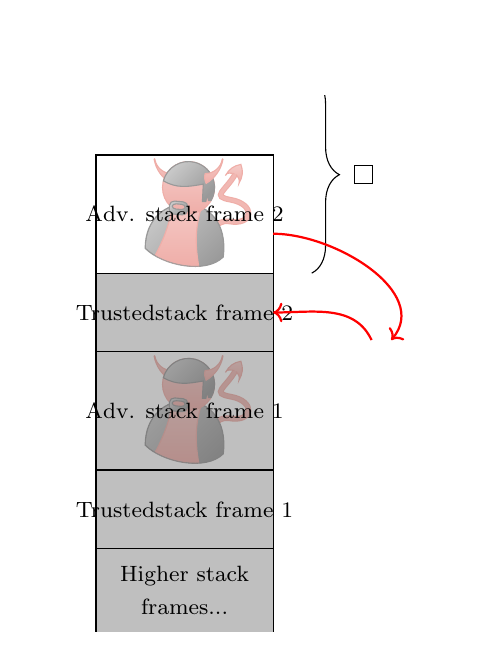
\begin{tikzpicture}[scale=.5, every node={scale=.5}]
      % recurrent parts
      \stdstackstart[13]
      \inactsf{(0,2)}{(4.5,4)} {\footnotesize Trusted\\ \footnotesize stack frame 1}
      \inactadv{(0,4)}{(4.5,7)} {\footnotesize Adv. stack frame 1}
      \inactsf{(0,7)}{(4.5,9)} {\footnotesize Trusted \\ \footnotesize stack frame 2}
      \actadv{(0,9)}{(4.5,12)} {\footnotesize Adv. stack frame 2}

      % Stack pointer 1
      \begin{scope}
        \clip (4.6,4) rectangle (9,13);
        \capbracebot{(4.6,4)}{(4.6,13.5)}{adv. stack\\\footnotesize cap. 1}
      \end{scope}
      Stack pointer 2
      \begin{scope}
        \clip (4.8,4) rectangle (9,13.5);
        \capbrace{(5.2,9)}{(5.2,14)}{adv. stack\\\footnotesize cap. 2}
      \end{scope}

      \draw[red,thick,->] (4.5,10) to[out=0,in=50] node[midway,right] {} (7.5,7.3);
      \draw[red,thick,->] (7,7.3) to[out=115,in=0] node[midway,right] {} (4.5,8);
    \end{tikzpicture}
    \caption{An adversary uses a previous stack frame's stack pointer.}
    \label{fig:stack-ptr-abuse}
  \end{subfigure}
  \begin{subfigure}{0.49\linewidth}
    \centering
    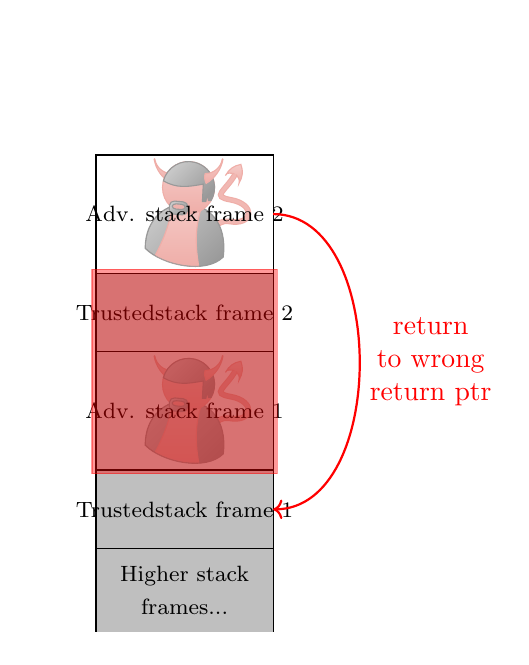
\begin{tikzpicture}[scale=.5, every node={scale=.5}]
      % recurrent parts
      \stdstackstart[13]
      \inactsf{(0,2)}{(4.5,4)} {\footnotesize Trusted\\ \footnotesize stack frame 1}
      \inactadv{(0,4)}{(4.5,7)} {\footnotesize Adv. stack frame 1}
      \inactsf{(0,7)}{(4.5,9)} {\footnotesize Trusted \\ \footnotesize stack frame 2}
      \actadv{(0,9)}{(4.5,12)} {\footnotesize Adv. stack frame 2}
      \fill[red,draw=red,opacity=.4] (-.1,3.9) rectangle (4.6,9.1);
      \draw[red,thick,->] (4.5,10.5) to[out=0,in=0] node[midway,right,align=center] {return\\ to wrong\\ return ptr} (4.5,3);
    \end{tikzpicture}
    \caption{An adversary jumps to a previous stack frame's stack pointer.}
    \label{fig:ret-ptr-abuse}
  \end{subfigure}
  
  \caption{Possible ways to abuse stack and return capabilities}
  \label{fig:stack-ret-ptr-abuse}
\end{figure}

Our StackTokens calling convention is based on a traditional single stack, shared between all components.
As we are on a capability machine, it is natural to add some extra protection to stack and return pointers.
First, we replace stack pointers with stack capabilities.
When a new stack frame is created, the caller provisions it with a stack capability, restricted to the appropriate range, i.e.\ it does not cover the caller's stack frame.
Return pointers, on the other hand, are replaced by a sealed pair of return capabilities.
They form an opaque closure that the callee can only jump to, and the caller's data becomes available to the caller's return code. 

While the above adds extra protection, it is important to understand that the above is not sufficient for enforcing WBCF and LSE.
While adversaries only get access to capabilities that they are allowed to use during the stack frame, they have ways to store these capabilities and use them when they are no longer allowed to do so.
Figure~\ref{fig:stack-ret-ptr-abuse} illustrates two examples of this.
The figure on the left (Figure~\ref{fig:stack-ptr-abuse}) blabla

\begin{itemize}
\item informally explain how an adversary may try to abuse stack and return caps
\item informally explain how we prevent this using linear capabilities
\item use the tikz pictures from the PriSC presentation to explain all of this
\end{itemize}
\section{A Capability Machine with Sealing and Linear Capabilities}
\begin{itemize}
\item present our target language and its operational semantics (excerpts)
\item mention roughly what components look like
\end{itemize}
\section{Formulating Security with a Fully Abstract Overlay Semantics}
\begin{itemize}
\item present our source language, its operational semantics (excerpts)
\item mention our assumption of reasonability
\item present the full abstraction theorem.
\item sketch high-level structure of the proof
\end{itemize}
\section{Discussion}
\begin{itemize}
\item mention that tail calls are supported through xcall
\item explain how fully abstract overlay semantics could form one pass of a verified secure compiler.
\end{itemize}
\section{Related Work}
\begin{itemize}
\item CFI and friends
\item our ESOP 2018 paper \citep{skorstengaard_reasoning_2017}
\item undefined behavior and full abstraction \citep{juglaret_beyond_2016}
\end{itemize}
\bibliography{references}


%% Appendix
% \appendix
% \section{Appendix}

% Text of appendix \ldots

\end{document}
